\documentclass[12pt,a4paper]{article}
\usepackage{algorithm, algpseudocode, amsmath, amssymb, amsthm, bm, csquotes, emf, empheq, geometry, graphicx, hyperref, listings, mhchem, multirow, siunitx, caption, float, longtable}
\usepackage[italicdiff]{physics}
\usepackage[section]{placeins}
\usepackage[justification=centering]{caption}
\usepackage[column=O]{cellspace}
% \usepackage[extrafootnotefeatures]{xepersian}
\hypersetup{colorlinks=true, urlcolor=cyan}

\title{Molecular Dynamics}

\author{Zahra Akbari}

\date{}


% \settextfont{}
\linespread{1.2}

\setlength\cellspacetoplimit{5pt}
\setlength\cellspacebottomlimit{3pt}
\newcommand{\multlinecell}[1]{\begin{tabular}[c]{@{}c@{}}#1\end{tabular}}

\newcommand{\qfrac}[2]{\left(\frac{#1}{#2}\right)}
\newcommand{\fsqrt}[2]{\sqrt{\frac{#1}{#2}}}
\newcommand{\ddfrac}[2]{{\displaystyle\frac{\displaystyle #1}{\displaystyle #2}}}
\newcommand{\pdvc}[3]{\qfrac{\partial #1}{\partial #2}_{#3}}
\newcommand{\dbar}{{d\mkern-7mu\mathchar'26\mkern-2mu}}
\newcommand*{\defeq}{\mathrel{\vcenter{\baselineskip0.5ex \lineskiplimit0pt
			\hbox{\scriptsize.}\hbox{\scriptsize.}}}
	=}

\begin{document}
	\maketitle
	\section*{Theory }
	100 particles is placed in a crystal lattice in the left side of 30 by 30 box. Calculating the Force using the Lennard jones formula:
	\begin{align*}
		F = \sigma (\frac{-6}{r^7}-\frac{-12}{r^{13}})
	\end{align*}
	The system trajectory is obtained by velocity verlet diffrential solving method. Reduced units are used for faster simulations.

	
% \pagebreak


	\section*{Results}
	The initial states is shown below:
	\begin{figure}[H]
		\centering
		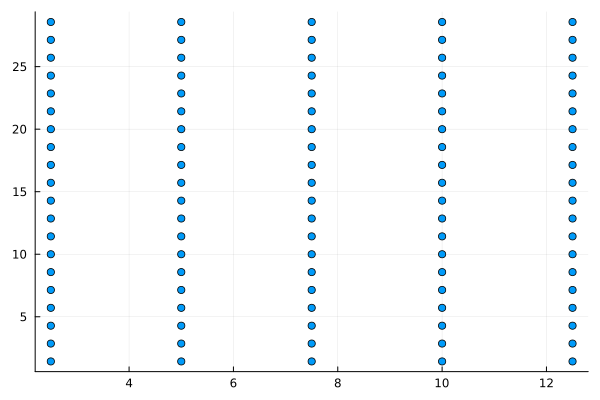
\includegraphics[width=10cm]{box0.png}
		\caption{crystal lattice }

	\end{figure}

	after 3000 velocity verlet step the system would look like this:
	
	\begin{figure}[H]
		\centering
		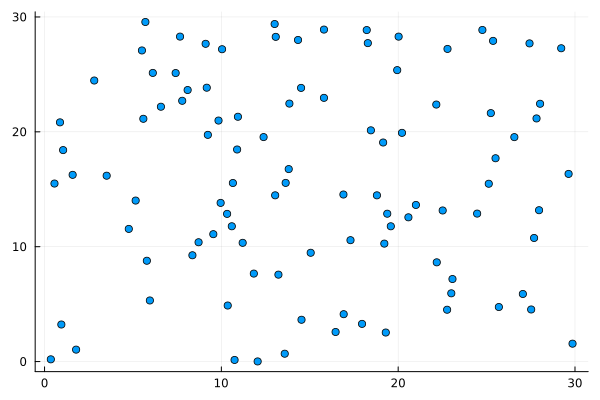
\includegraphics[width=10cm]{boxafter3000.png}
		\caption{the state after 3000 velocity verlet steps. }
	\end{figure}
	The gif is also available in the attached files.
	The number of molecules in the left side over time is plotted.
	\begin{figure}[H]
		\centering
		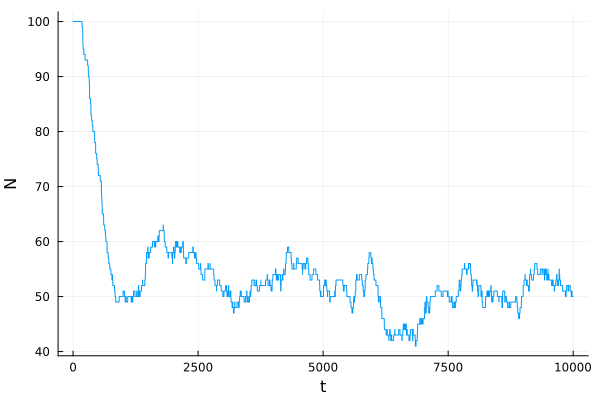
\includegraphics[width=10cm]{n.png}

		\caption{Number of Molecules in the left side after 10000 steps. }
	\end{figure}
		We analyze the energy conservation by saving the Lennard jones potential in VelVerlet function. The result is shown below:
		\begin{figure}[H]
			\centering
			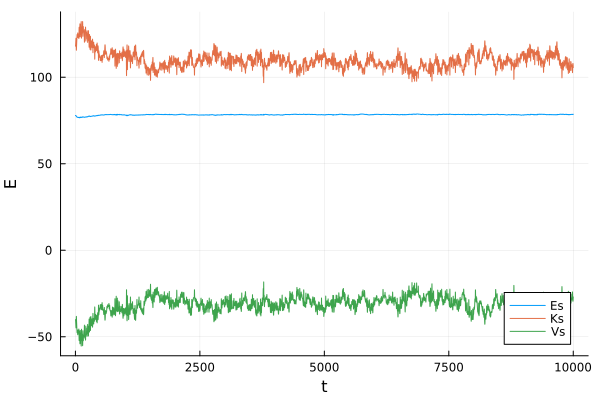
\includegraphics[width=10cm]{E.png}
			\caption{Energy conservation}
		\end{figure}
		Auto-Correlation of velocities is also calculated:
		\begin{figure}[H]
			\centering
			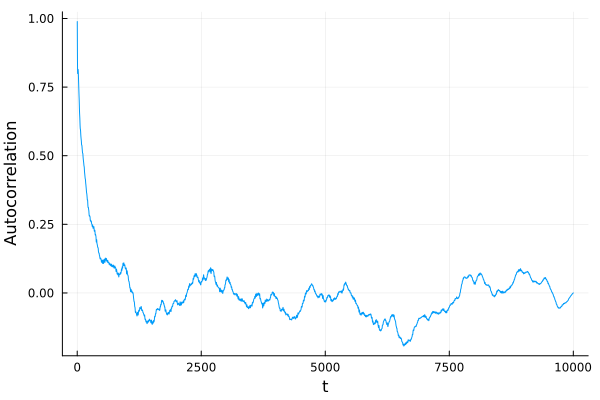
\includegraphics[width=10cm]{auto.png}
			\caption{Auto-Correlation of velocities}
		\end{figure}
		Temperature is calculated useing kinetic energy:
		\begin{figure}[H]
			\centering
			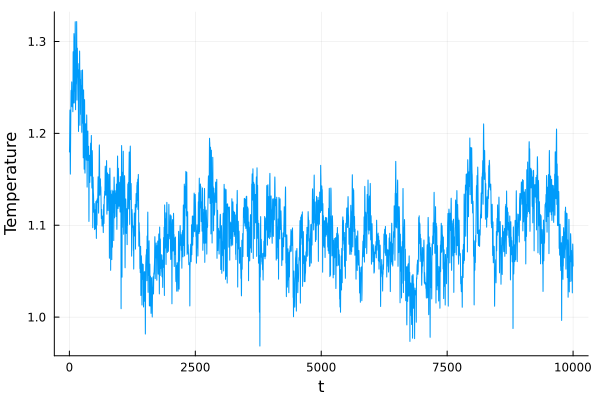
\includegraphics[width=10cm]{T.png}
			\caption{Temperature over time step}
		\end{figure}
		Pressure is calculated using virial theoream:
		\begin{align*}
			P = \frac{NkT}{V} - \frac{\sum_{i}^{} F_i.r_i}{3V}
		\end{align*}
		\begin{figure}[H]
			\centering
			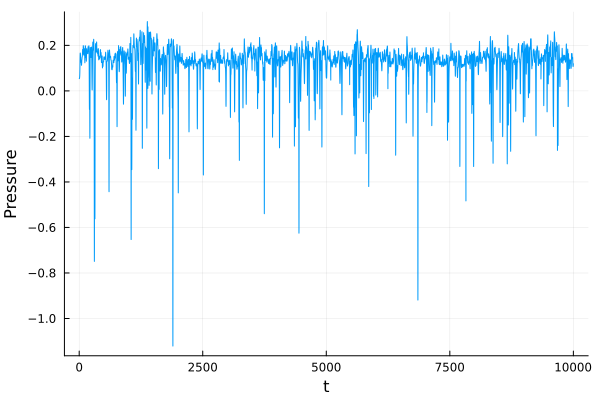
\includegraphics[width=10cm]{P.png}
			\caption{Pressure over time step}
		\end{figure}
		fiting a line to P over T graph we aim to find the Wan der Vaals coefficents.
		\begin{figure}[H]
			\centering
			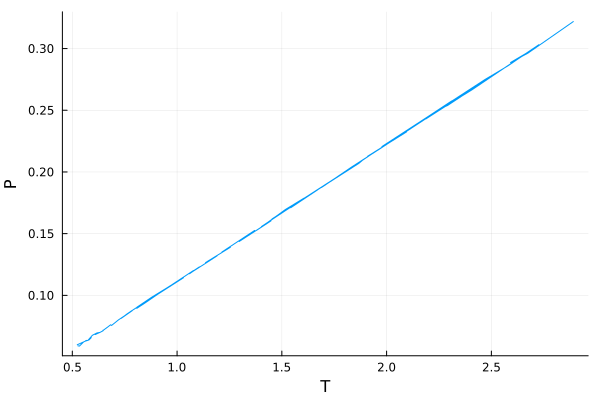
\includegraphics[width=10cm]{Pt.png}
			\caption{Pressure over Temperature after 50 millions velocity verlet steps.}
		\end{figure}
		\begin{align*}
			slope &=  0.11101 \\
			intercept &= 0.00023 
		\end{align*} 
		Phase transition is observes scaling the velocities by 0.5 coefficent every 100 steps for 10000 velocities verlet steps.
		\begin{figure}[H]
			\centering
			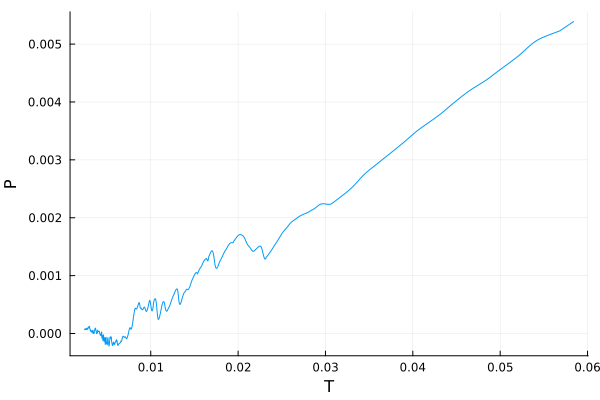
\includegraphics[width=10cm]{phase.png}
			\caption{Phase transition in P-T diagram}
		\end{figure}

		\end{document}
	